\chapter{Requirements}

\section{Functional requirements}

\subsection{Data Integration}

The Data Integration part of the platform needs to integrate several data sources to the Journal. Integration means that it must be able 
to detect the changes made to the data, and push events that can be either create event or update event or delete event.
In the following, we call a data entry a \textit{resource}. A resource is a keyed data defined by its id (for example \verb|/client/1| for a
resource of type client of id 1). Each type of resource has a defined set of fields (for example a client
will have a field name, address, ...).
\\

More specifically, the platform needs to integrate several data source that exposes REST API. Such API exposes information
concerning business data such as new sales information, new financial information, new production information...
Each time that a resource is modified in one of these data sources, the platform should detect this change, create from it
the corresponding event and push it into the Journal.

The problem with most REST APIs is that they are not evented, i.e they are pulled-based and not pushed-based. 
One must sent an HTTP request to query new data each time they need to. There exists some techniques to stream data via HTTP 1.1 and the 
Chunked Transfer Encoding, but the REST APIs that the platform needs to integrate does not exposes such stream interface. 
Thus, the architecture of this part needs to provide a way to perform incremental pull from data sources, and then transform
it in a push stream of events towards the Journal.


\subsection{Journal and Stream Processing}

The Journal must provide a way for data producers to push one or several events that represents the creation, update or 
delete of a resource. Moreover, it must allows data consumers to subscribe to the stream of inserted events. Events must be
immutable and are stored in a sequence that respects the insertion order. The stream of events pushed to the data consumers
(stream processors) must be in the same order than the insertion order and with no event loss. Of course, the Journal must be persistent to
be able to recover its data after a shutdown or crash of the platform.
\\

The Stream Processing part is the most complex part of the platform. This part should be a library that allows the user
to define a tree a stream processors (see Figure \ref{fig:tree}), where the root of the tree is the Journal. 

\begin{figure}[h]
  \begin{center} 
    \makebox[\textwidth]{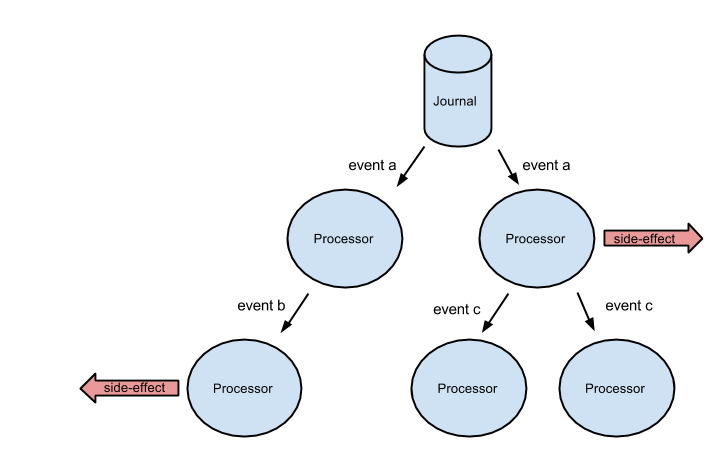
\includegraphics[width=1.0\textwidth]{img/tree.png}}
    \caption{A tree of stream processors}
    \label{fig:tree}
  \end{center}
\end{figure}

A stream processor receives events coming from its parent node. Upon the receive of an event, it can do one or several of these
actions (see Figure \ref{fig:streamprocessor}):
\begin{itemize}
  \item Creation of a sub-stream: the stream processor can transform a received event to a stream (several events), creating a sub-stream
  inside the global stream. The sub-stream must be inserted in-place in the stream: the whole sub-stream should be
  send in-order to the node's children before processing the next incoming event (see Figure \ref{fig:substream}).
  The user implementing this method, called \verb|process|, must ensure that the function is pure (without side-effect).
  The user must also be aware that the function may be call several times for an event (at-least-once process semantic).
  \item Side-effect with exactly-once semantics: The second action possible is to perform a side-effect upon each of the event
  of the sub-stream generated by the \verb|process| method. This side-effect can be for example updating a database representing
  a derived view on the data. This method, called \verb|performSideEffect|, has a exactly-once semantic, so the user
  can define non-idempotent side-effects. Nevertheless, the user must ensure that the side-effect is atomic. 
\end{itemize}

\begin{figure}[h]
  \begin{center} 
    \makebox[\textwidth]{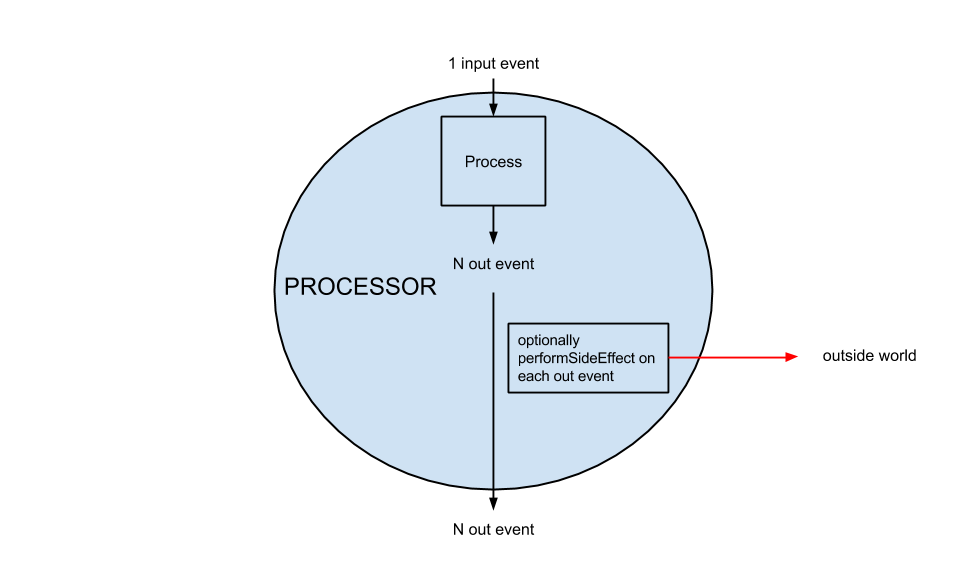
\includegraphics[width=1.0\textwidth]{img/stream_processor.png}}
    \caption{A stream processor}
    \label{fig:streamprocessor}
  \end{center}
\end{figure}

\begin{figure}[h]
  \begin{center} 
    \makebox[\textwidth]{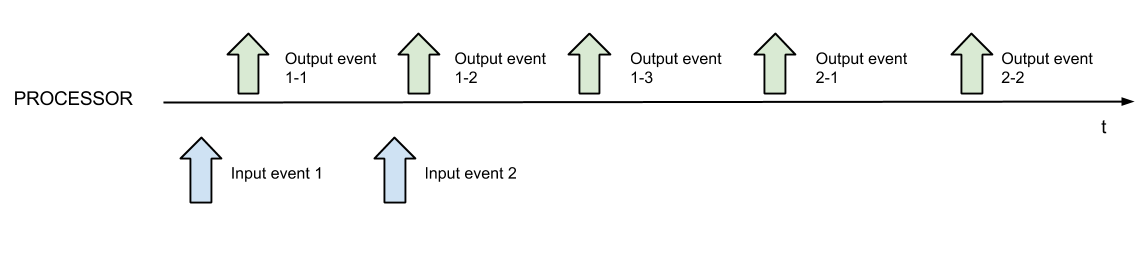
\includegraphics[width=1.0\textwidth]{img/substream.png}}
    \caption{In-order insertion of a substream in a stream}
    \label{fig:substream}
  \end{center}
\end{figure}

Another important functional requirements for the processor is that the \verb|process| and \verb|performSideEffect| methods is that they can ensure the
sequentiality of asynchronous non-blocking operations (for example, a side-effect or a process can be done via an asynchronous call to a 
database, but despite the asynchronous nature of the call, the processor must wait that the asynchronous call has returned
before processing the next event).


